% \documentclass{article}
\documentclass[fleqn]{article}

\usepackage{notations}
\usepackage{amsfonts}
\usepackage{amsmath}
\usepackage{relsize}
\usepackage{geometry}


\geometry{
 a4paper,
 total={170mm,257mm},
 left=20mm,
 top=20mm,
 }

% ======================================================================================================================
% NOTATIONS
% ======================================================================================================================

% ======================================================================================================================
% NOTATIONS
% ======================================================================================================================

% \setlength{\mathindent}{0pt}
\setlength{\parindent}{0em}
\setlength{\parskip}{1em}
\renewcommand{\baselinestretch}{1.0}

\title{\texttt{PytHHOn3D} documentation}
\author{David Siedel \and Olivier Fandeur \and  Thomas Helfer}

\date{01/08/2020}




% ======================================================================================================================
% DOCUMENT
% ======================================================================================================================

\begin{document}

  \maketitle

  \section{Notations}

    \begin{itemize}
      \item $a$ denotes a scalar value, usually a parameter, a real number, etc.
      \item $\tensoro{a}$ denotes a $0$-th order tensor-valued function.
      \item $\tensori{a} = \begin{pmatrix}
        \tensoro{a}_1 \\ \vdots \\ \tensoro{a}_n
      \end{pmatrix}$ denotes a $1$-st order tensor-valued function.
      \item $\tensorii{a} = \begin{pmatrix}
        \tensoro{a}_{11} & \dots & \tensoro{a}_{1n} \\ \vdots & \ddots & \vdots \\ \tensoro{a}_{N1} & \dots & \tensoro{a}_{Nn}
      \end{pmatrix}$ denotes a $2$-nd order tensor-valued function.
      \item $\tensoriv{a}$ denotes a $4$-th order tensor-valued function.
      \item $\tensorii{a}^t$ denotes the transpose of $\tensorii{a}$
    \end{itemize}

    \newpage
    
  \section{Model problem}

        Let a solid represented by $\Omega \subset \mathbb{R}^d$ a closed domain with Lipschitz boundary $\partial \Omega \subset \mathbb{R}^{d-1}$.
        \\
        The solid morphs through the action of volumetric forces in its inner body, and through the influence of contacts forces and imposed displacements at its surface.
        \par

        Let $\partial \Omega = \partial \Omega_N \oplus \partial \Omega_D$ with $\partial \Omega_N \subset \partial \Omega$ the boundary of the body subjected to contact forces (\textit{i.e.} subjected to Neumann boundary conditions), and $\partial \Omega_D \subset \partial \Omega$ the boundary of the body subjected to imposed displacements (\textit{i.e.} subjected to Dirichlet boundary conditions).
        \par

        Let $\tensori{t}\subscript{N} \in L^2(\partial \Omega_N;\Rd)$ contact forces acting on $\partial \Omega_N$ and $\tensori{u}\subscript{D} \in L^2(\partial \Omega_D;\Rd)$ imposed displacements acting on $\partial \Omega_D$
        \par

        Let $\tensori{f} \in L^2(\Omega; \Rd)$ volumetric forces acting in $\Omega$.
        \par

        Let $\tensori{u} \in \Hone$ denote the displacement field in $\Omega$ and $\tensorii{\sigma} \in \Hdiv$ the stress tensor field such that $\tensorii{\sigma} = \tensoriv{A} : \nabla \tensori{u}$ where the fourth-order stiffness tensor $\tensoriv{A}$ is reprensentative of the behavior law of the material, and thus depends on time, displacement, internal variables, damamge, etc.
        \par

        The model problem in solid mechanics reads : find $\tensori{u} \in \Hone$ the displacement field in $\Omega$, such that

        \begin{equation}
          \begin{array}{ll}
            \nabla \cdot \tensorii{\sigma} = \nabla \cdot (\tensoriv{A} : \nabla \tensori{u}) =  - \tensori{f} & \mbox{in $\Omega$}
            \\
            \tensorii{\sigma} \cdot \tensori{n} = (\tensoriv{A} : \nabla \tensori{u}) \cdot \tensori{n} = \tensori{t}\subscript{N} & \mbox{on $\partial \Omega_N$}
            \\
            \tensori{u} = \tensori{u} \subscript{D} & \mbox{on $\partial \Omega_D$}
          \end{array}
          \label{eq_strong_problem}
        \end{equation}
        \par

        The weak form of \eqref{eq_strong_problem} reads : find $\tensori{u} \in \Hone$ the displacement field in $\Omega$, such that

        \begin{equation}
          \begin{array}{ll}
            \displaystyle
            \int_{\Omega} \nabla \tensori{v} : \tensoriv{A} : \nabla \tensori{u} = \int_{\Omega} \tensori{v} \cdot \tensori{f} + \int_{\partial \Omega_N} \tensori{v} \cdot \tensori{t}\subscript{N} & \forall \tensori{v} \in \Hone
            \\
            \tensori{u} = \tensori{u} \subscript{D} & \mbox{on $\partial \Omega_D$}
          \end{array}
          \label{eq_weak_problem}
        \end{equation}
  
  \newpage

  \section{The Galerkin method}

    \subsection{Discretization}
      
      % The Finite Element (FE) method consists in discretizing the problem both geometrically and functionally :

      \subsubsection{Spatial discretization}
      
        $\Omega$ which is a continuum, is partitioned into simplistic shapes, called elements, which are triangles or
        quandrangles when $d = 2$ and tetrahedra, hexahedra or prisms when $d = 3$.
        The resulting partition of $\Omega$ is the mesh $\Mesh(\Omega)$ of $\Omega$, where $h$ denotes the diameter of
        the largest element $T$ in $\Mesh(\Omega)$

        \begin{infobox}{admissible shapes}
          Only such simplistic shapes are admissible, because the FE method lies on the use of the Lagrange polynomial basis (see \ref{sec_functional_discretization}), and more complex shapes, such as general polytopes, are not practicable with such a polynomial basis.
        \end{infobox}

      \subsubsection{Functional discretization}
      \label{sec_functional_discretization}
        
        The functional space where the solution to $\eqref{eq_weak_problem}$ lives, $\Hone$, which is of infinite dimension, is approximated by a subset $V \subset \Hone$ of finite dimension.
        By approximating $\Hone$ with a finite-dimension space $V$, one can define a basis on $V$ (since $V$ is hilbertian, as a subspace of the hilbertian space $\Hone$), and thus express any function in $V$ as a linear combination of the functions constituing the basis of $V$. It is then possible to search for candidates to solutions to \eqref{eq_weak_problem} in $V$, and hence to write
        \eqref{eq_weak_problem} in an algebraic form, using the decomposition of any function in $V$ in its basis.
        \par
        A convinient choice for $V$ is the Galerkin approximation space :

        \begin{equation}
          \displaystyle
          \Pkapprox =
            \Bigg\{
            \tensori{v} \in \mathcal{C}^0(\Omega;\Rd)
            \ \ \Bigg\vert \ \ 
            \forall T \in \Mesh(\Omega), \tensori{v} \vert_{T} \in \mathbb{P}^k(T;\Rd)
            \Bigg\}
        \end{equation}

        \begin{infobox}{Conformal approximation of the solution}
          As the unknown in \eqref{eq_weak_problem} is the displacement field in the body represented by $\Omega$, it is natural to consider continuous functions for $V$, since $\Omega$ is a continuum (and so is the displacement of the matter conctituting $\Omega$).
        \end{infobox}

    \subsection{Algebraic formulation}
    \label{sec_algebraic_formulation}
    
        % The FE (or Galerkin) method consists in finding $\Pi_{V}(\tensori{u})$ the projection of $\tensori{u}$ onto $V$. As $\Pi_{V}(\tensori{u}) \in V$, finding $\Pi_{V}(\tensori{u})$ amounts to finding its coeficients in $\mathcal{B}_V$.

      \subsubsection{Algebraic formulation : vectorial representation of a function}
      \label{sec_algebraic_formulation_1}
      
        Let $V \subset L^2(\Omega;\mathbb{R})$ an hilbertian space of scalar-valued functions, with finite dimension $N_V$. Let $V^d \subset L^2(\Omega;\Rd)$ the product of $V$ times the problem dimension $d$, \textit{i.e.} the space of $d$-valued functions such that for each direction $1 \leq i \leq d$, the component $\tensoro{v}\subscript{i}$  along the $i$-th direction of any function $\tensori{v} \in V^d$ is in $V$. The dimension of $V^d$ is then :
        \begin{equation}
          N_V^d = d \cdot N_V
        \end{equation}
        \par
        Let $\mathcal{B}_V$ a basis in $V$, such that $\mathcal{B}_V = (\tensoro{\beta}\subscript{m})\subscript{1 \leq m \leq N_V}$.
        \newline
        Any function $\tensoro{v}\subscript{i} \in V$ can be expressed as a linear combination of all vectors $\tensoro{\beta}\subscript{m} \in \mathcal{B}_V$, such that, for $1 \leq i \leq d $ :

        \begin{equation*}
          {\tensoro{v}\subscript{i}} = \sum_{1 \leq m \leq N_V} {v}\subsupscript{i}{m} \cdot \tensoro{\beta}\subscript{m}
          =
          \tensoro{\bbbeta} \cdot \tensoro{\mathbbl{v}}\subscript{i}
          =
          \tensoro{\bbbeta} \supscript{t} \times \tensoro{\mathbbl{v}}\subscript{i}
          \mbox{ with }
          \tensoro{\mathbbl{v}}\subscript{i} =
          \begin{pmatrix}
            {v}\subsupscript{i}{1} \\ \vdots \\ {v}\subsupscript{i}{N_V}
          \end{pmatrix} \in \mathbb{R}^{N_V \times 1}
          \mbox{ and }
          \tensoro{\bbbeta} =
          \begin{pmatrix}
            \tensoro{\beta}\subscript{1} \\ \vdots \\ \tensoro{\beta}\subscript{N_V}
          \end{pmatrix} \in V^{N_V \times 1}
        \end{equation*}

        Finally, the vector $\tensori{v}$ writes as the scalar product of the vectors formed by $(\mathbbl{v}\subscript{i})\subscript{1 \leq i \leq d}$ and $(\bbbeta)\subscript{1 \leq i \leq d}$ :
        
        \begin{equation*}
          \tensori{v} = \tensori{\bbbeta} \supscript{t} \times \tensori{\mathbbl{v}}
          \mbox{ with }
          \tensori{\mathbbl{v}} = 
          \begin{pmatrix}
            \mathbbl{v}\subscript{1} \\ \vdots \\ \mathbbl{v}\subscript{d}
          \end{pmatrix} \in \mathbb{R}^{N_V^d \times 1}
          \mbox{ and }
          \tensori{\bbbeta} = 
          \begin{pmatrix}
            \bbbeta \\ \vdots \\ \bbbeta
          \end{pmatrix} \in V^{N_V^d \times 1}
        \end{equation*}

      \subsubsection{Algebraic formulation : matricial representation of the gradient}

        Let specify $V$ in $\mathbb{P}^k(\Omega;\mathbb{R})$ with finite dimension $N_V$, endowed with a basis $\mathcal{B}_V$. The gradient operator $\nabla$ in $V$ is the linear application that acts on any $\tensoro{v} \in V$, and projetcs onto $V' = \nabla \mathbb{P}^k(\Omega;\mathbb{R})$ of dimension $N_{V'}$.
        \par
        Since the derivative of a polynomial of order $k$ writes as a linear combination of polynomials of order $k-1$, the derivative $\tensoro{v}\subscript{i,j}$ of the $i$-th component of $\tensori{v}$ along the $j$-th direction writes as :
        \begin{equation*}
          \tensoro{v}\subscript{i,j} = \tensoro{\bbbeta}\supscript{t} \times \tensoro{\mathbbl{v}}\subscript{ij}
          \mbox{ where }
          \tensoro{\mathbbl{v}}\subscript{ij} = \tensoro{\mathbbl{B}}\subscript{j} \times \tensoro{\mathbbl{v}}\subscript{i}
          \mbox{ and }
          \tensoro{\mathbbl{B}}\subscript{j} \in \mathbb{R}^{N_V \times N_{V'}}
        \end{equation*}

        $\tensoro{\mathbbl{B}}\subscript{j}$ is the matrix that returns the coeficients of the derivative of a polynomial in $\mathcal{B}_V$ along the $j$-th direction.
        \par
        The matrix $(\tensoro{\mathbbl{v}}\subscript{ij})\subscript{1 \leq i,j \leq d}$ can be expressed as a vector $\tensori{\mathbbl{v}}\supscript{\nabla} = (\tensoro{\mathbbl{v}}\subscript{s})\subscript{1 \leq s \leq d^2}$ using a multi-index notation $\mathfrak{n} : \llbracket 1,d^2 \rrbracket \supset s \mapsto i(s), j(s) \subset \mathbb{N}^2$ :

        \begin{equation*}
          \tensori{\mathbbl{v}}\supscript{\nabla}
          =
          \tensorii{\mathbbl{B}}
          \times
          \tensori{\mathbbl{v}}
          \mbox{ with }
          \tensorii{\mathbbl{B}} = (\mathbbl{B}\subscript{j(s)})\subscript{1 \leq s \leq d^2} \in \mathbb{R}^{N_V \times d^2 N_{V'}}
        \end{equation*}

        \begin{infobox}{isoparametric elements and derivation}
          $\tensorii{\mathbbl{B}}$ is then the matricial representation of the gradient operator in the polynomial space.
          In the context of the FE method, a mapping from a reference frame to a deformed frame is used to compute the derivative of shape functions in isoparametric elements. this mapping intervenes as an intermediate appplication in the process of derivation (\textit{i.e.} the $\tensorii{\mathbbl{B}}$ matrix is multpiplied by another matrix, namely the mapping matrix), but it does not change the algebraic feature of the gradient operator, as presented above.
        \end{infobox}

        \begin{infobox}{polynomial order of the derivative}
          As mentioned, the derivative of a function $\tensoro{v}$ in $V$ is an order inferior to that of $\tensoro{v}$. From a mechnaical standpoint, this means that if the displacement is apporximated by a polynomial of order $k$, the deformation (and hence the stress) is a polynomial of order $k-1$ : some accuracy on the approximation in the stress space is lost in this manner.
        \end{infobox}

        In the special case when the symmetric gradient operator $\nabla^s$ is considered instead of the regular gradient operator $\nabla$, indicies corresponding to the lower triangular part of $\nabla^s$ are the same as those in the upper triangular part, and the notation is symplified.
        \newline
        Another, shorter, multi index notation $s' \mapsto i(s'), j(s')$ is used (\textit{i.e.} the Voigt notation), and the symmetry of $\nabla^s$ is implemented such that :

        \begin{equation*}
          \mathbbl{B}\subscript{j(s')} = 
          \begin{cases}
            \mathbbl{B}\subscript{j(s')} & \mbox{if } j(s') = i(s')
            \\
            1/2 \cdot \mathbbl{B}\subscript{j(s')} + 1/2 \cdot \mathbbl{B}\subscript{i(s')} & \mbox{if } j(s') \neq i(s')
          \end{cases}
        \end{equation*}

      \subsubsection{Algebraic formulation in an element}

        Let $T \in \Mesh(\Omega)$. Let $\mathcal{B}_T$ a basis on $\mathbb{P}^k(T;\mathbb{R})$, of dimension $N_T$.
        Let $N_T^d = d \cdot N_T$ the dimension of the unknown vector in the element $T$.
        \par
        Using the algebraic formulation defined in \ref{sec_algebraic_formulation} :
        \begin{equation*}
          \nabla \tensori{{u}}
          =
          \tensori{\bbtheta}\supscript{t} \times \tensori{\mathbbl{u}}\supscript{\nabla}
          =
          \tensori{\bbtheta}\supscript{t} \times (\tensorii{\mathbbl{B}} \times \tensori{\mathbbl{u}})
          \mbox{ and }
          \nabla \tensori{{v}}
          =
          \tensori{\bbtheta}\supscript{t} \times \tensori{\mathbbl{v}}\supscript{\nabla}
          =
          \tensori{\bbtheta}\supscript{t} \times (\tensorii{\mathbbl{B}} \times \tensori{\mathbbl{v}})
        \end{equation*}

        Let $\tensorii{\mathbbl{M}}$ the mass matrix in $\mathbb{R}^{d \cdot N_T^d \times d \cdot N_T^d}$ such that
        $
          \tensorii{\mathbbl{M}} = (\tensoro{\mathbbl{M}} = \tensoro{\bbtheta} \times \tensoro{\bbtheta}\supscript{t})\subscript{1 \leq i,j \leq d}
        $

        Let $\tensoriv{\mathbbl{A}}$ the matrix in $\mathbb{R}^{d^2 \cdot N_T^d \times d^2 \cdot N_T^d}$ such that :

        \begin{equation*}
          \tensoriv{\mathbbl{A}} = (\tensoriv{A}\subscript{mn} \cdot \tensoro{\mathbbl{M}})\subscript{1 \leq m,n \leq d}
          \mbox{ where $m = \mathfrak{n}^{-1}(i,j)$ and $n = \mathfrak{n}^{-1}(k,l)$ are multi-indices for $\tensoriv{A}\subscript{ijkl}$}
        \end{equation*}

        The PVW in \eqref{eq_weak_problem} in the element $T$ writes in algebraic form as :

        \begin{equation}
            \int_T \tensori{\mathbbl{v}}\supscript{t} \times \tensorii{\mathbbl{B}}\supscript{t} \times \tensoriv{\mathbbl{A}} \times \tensorii{\mathbbl{B}} \times \tensori{\mathbbl{u}}
            =
            \int_T \tensori{\mathbbl{v}}\supscript{t} \times \tensorii{\mathbbl{M}} \times \tensori{\mathbbl{f}}
            +
            \int_{\partial T_N} \tensori{\mathbbl{v}}\supscript{t} \times \tensorii{\mathbbl{M}} \times \tensori{\mathbbl{t}}\subscript{N}
            \label{eq_weak_problem_algebraic}
        \end{equation}

        Using a quadrature rule $Q$ over $T$, \eqref{eq_weak_problem_algebraic} becomes :

        \begin{equation}
            \sum_{x_Q} \tensori{\mathbbl{v}}\supscript{t} \times \tensorii{\mathbbl{B}}\supscript{t} \times \tensoriv{\mathbbl{A}}(x_Q) \times \tensorii{\mathbbl{B}} \times \tensori{\mathbbl{u}}
            =
            \sum_{x_Q} \tensori{\mathbbl{v}}\supscript{t} \times \tensorii{\mathbbl{M}}(x_Q) \times \tensori{\mathbbl{f}}
            +
            \sum_{x_{Q_N}} \tensori{\mathbbl{v}}\supscript{t} \times \tensorii{\mathbbl{M}}(x_{Q_N}) \times \tensori{\mathbbl{t}}\subscript{N}
        \end{equation}

        One can define :

        \begin{equation*}
            \begin{array}{ll}
                \tensorii{\mathbbl{K}} = \sum_{x_Q} \tensorii{\mathbbl{B}}\supscript{t} \times \tensoriv{\mathbbl{A}}(x_Q) \times \tensorii{\mathbbl{B}} & \mbox{the stifness matrix in $T$}
                \\
                \tensori{\mathbbl{b}} = \sum_{x_Q} \tensorii{\mathbbl{M}}(x_Q) \times \tensori{\mathbbl{f}} + \sum_{x_{Q_N}} \tensorii{\mathbbl{M}}(x_{Q_N}) \times \tensori{\mathbbl{t}}\subscript{N} & \mbox{the external forces vector in $T$}
            \end{array}
        \end{equation*}

        And the vector of unknowns solution to \eqref{eq_weak_problem} is then :

        \begin{equation*}
            \tensori{\mathbbl{u}} = \tensorii{\mathbbl{K}}\supscript{-1} \times \tensori{\mathbbl{b}}
        \end{equation*}

  \newpage
  
  \section{The HHO method}

    \subsection{Functional space for the HHO method}

        The HHO method is a so-called "non-conformal method" (as opposed to conformal ones, among which is the Galerkin method, and by extension the standard FE method). The main feature of non-conformal method lies on the foundation of the intepretation of the problem \eqref{eq_weak_problem}.
        \newline
        As mentioned above, the Galerkin method consists in discretizing \eqref{eq_weak_problem} in a subspace of the original functional space, namely $\Hone$. This feature ensures that all theoretical results valid in $\Hone$ (Lax milgram theorem, Cea theorem, etc) are \textit{de facto} valid in the chosen finte dimensional subspace.
        \newline
        Non conformal method differ from conformal ones, in the sense that they seek the solution to \eqref{eq_weak_problem} in a superspace of $\Hone$, namely the broken Sobolev space $\Hbroken \supset \Hone$ :

        \begin{defbox}{Broken Sobolev space}
            \begin{equation}
                \Hbroken =
                \Bigg\{
                \tensori{u} \in L^2(\Omega;\Rd)
                \ \ \Bigg\vert \ \ 
                \forall T \in \Mesh(\Omega), \tensori{u} \vert_T \in H^1(T;\Rd)
                \Bigg\}
            \end{equation}
        \end{defbox}

        \subsubsection{Practical mechanical interpretation of the broken Sobolev space}

            From a physical standpoint, the broken Sobolev space of displacements in a body $\Omega$ defines an twisted, non-physical interpretation of matter, as if it was piece-wise continuous in the body $\Omega$, \textit{i.e.} as if the body $\Omega$ was made of patches of matter, that have \textit{a priori} no connection at all : if displacement over mesh belongs to $\Hone$, its interpretation in $\Hbroken$ is the union of all local displacements in each element (see \figref{fig_broken_sapce}), such that there are jumps of displacement between elements.
            
            \begin{figure}[h]
                \centering
                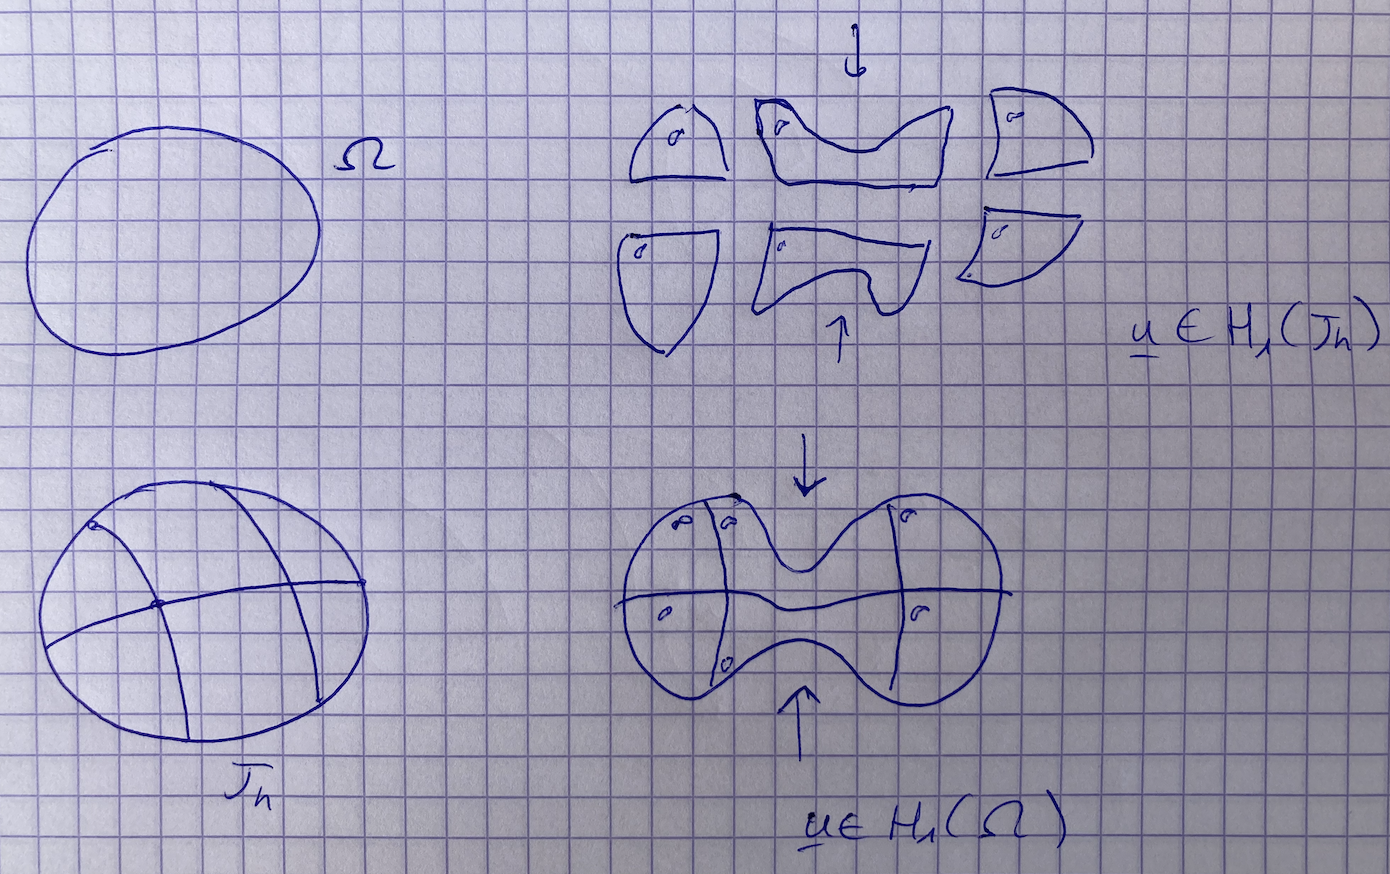
\includegraphics[width=10.cm]{img/broken_space1.png}
                \caption{illustration of displacement in the broken Sobolev space}
                \label{fig_broken_sapce}
            \end{figure}

            Mechanicallly, this amounts to endow each element of a mesh defined by the Galerkin method with a rigid body motion. The main reason for considering such broken spaces over conformal space is described in section [XXX]. However, applying directly the Galerkin method in such broken spaces is not valid (actually, the Galerkin method is by definition valid on subspaces on $\Hone$) : since the displacement is pieace-wise continuous, \textit{a priori} nothing ensures communication between elements. One could pull on a given element of the mesh without any influence on its neighbours.

            \subsubsection{From the non-physical broken Sobolev space towards a more physical one : weak form of continuity}

            To recover a physical behavior of matter, \textit{i.e.} a form of continuity on the displacement field, one needs to introduce another ingredient to the discontinuous displacement field. In order to do so, one introduces an elastic membrane defined on the skeleton of the mesh (\textit{i.e.} on the edges of the mesh) and that acts on all elements of the mesh to enforce a "pulling force" between each element and its neighbours. Hence, the broken mesh is patched back with this elastic membrane, such that all elements keep some free individual movement capacity, but influence their neighbours in their movement through the elastic membrane : the influence of the movement of an element on its neighbours depends then on the stiffness of the memembrane. In particular, taking an infinte stiffness corresponds to ensuring that no free movement is possible for elements, and so that the piece-wise continuous displacement field is actually globally continuous over the whole mesh.

            \begin{figure}[h]
                \centering
                \includegraphics[width=10.cm]{img/broken_space.png}
                \caption{illustration of displacement in the broken Sobolev space endowed with an elastic membrane}
                \label{fig_broken_sapce1}
            \end{figure}

            From a mathematical point of view, defining a pulling force between elements on the displacement field corresponds to enforce a penalization in the least square sense.


        % The HHO method, as well as the FE method, consists in discretizing \eqref{eq_weak_problem} both geometrically and functionally in order to actually compute approximated solutions that are not analytically reachable.
        % \par
        % Contrary to the FE method, the HHO method does not consider finding the solution in $\Hone$, but not in a richer space, namely the broken Sobolev space. Given, a mesh $\Mesh(\Omega)$ of $\Omega$ (see \ref{sec_mesh} for further description of what a mesh is within the framework of the HHO method), one defines the broken Sobolev space in the following way :

    \newpage

    \subsection{Mechanical intepretation and definition of the pulling force between elements}
        
        Let consider the skeleton $\mathcal{F}_h(\Omega)$:

        \begin{equation*}
            \mathcal{F}_h(\Omega) = \bigcup_{T \in \Mesh(\Omega)} \bigcup_{F \in \partial T} F
        \end{equation*}

        Let consider $\mathcal{T}_h(\Omega, \Gamma)$, the mesh of $\Omega$ based on $\Mesh(\Omega)$, such that faces in $\mathcal{F}_h(\Omega)$ are expended from $\mathbb{R}^{d-1}$ into $\Rd$ and form a domain $\Gamma \subset \Rd$ of dimension $h_\Gamma \times w_\Gamma$ :

        \begin{figure}
        \centering
        \begin{minipage}{.5\textwidth}
            \centering
            \includegraphics[width=4.cm]{img/membrane.png}
            \captionof{figure}{membrane 1}
            \label{fig_test1}
        \end{minipage}
        \begin{minipage}{.5\textwidth}
            \centering
            \includegraphics[width=4.cm]{img/membrane_2.png}
            \captionof{figure}{membrane 2}
            \label{fig_test2}
        \end{minipage}
        \end{figure}

        The membrane $\Gamma$ is made of a material of Young modulus $\beta$ and Poisson ratio $0$ : hence, the behavior tensor $\tensoriv{A}$ writes as $\tensoriv{A} = \beta \cdot \tensoriv{1}$ . Let consider two elements $T_1$ and $T_2$ made of undeformable bodies (since the displacement is defined up to a rigid body motion, as mentioned) linked with the membrane $\Gamma$. Let fix $T_1$ and pull on $T_2$. The elastic membrane is in equilibrium, hence all forces acting on it are equal, which writes as :

        \begin{equation*}
            \tensori{F}\subscript{T_1 \rightarrow \Gamma} = - \tensori{F}\subscript{T_2 \rightarrow \Gamma}
        \end{equation*}

        And 

        \begin{equation*}
            \tensori{F}\subscript{T_1 \rightarrow \Gamma} = \int_{\Gamma \cap T_1} \beta \cdot \tensoriv{1} : \nabla \tensori{u}\vert_{\Gamma \cap T_1} \cdot \tensori{n}
        \end{equation*}
        
        Writing the equilibrium of the membrane
  \end{document}